\documentclass{article}
\usepackage{amsthm, amsmath, tikz}
\usepackage[margin=1in]{geometry}
\begin{document}
    \noindent\textbf{Math 327 Homework 2}\hfill Anchu A. Lee\\\\
    
    \noindent\textbf{2.4}
    \begin{enumerate}
        \item $S = \{(1,1),(1,2),(1,3),(1,4),(1,5),(1,6),(2,1),(2,3),(2,4),(2,5),(2,6)\\
               (3,1),(3,2),(3,3),(3,4),(3,5),(3,6),(4,1),(4,2),(4,3),(4,4),(4,5),(4,6)\\
               (5,1),(5,2),(5,3),(5,4),(5,5),(5,6),(6,1),(6,2),(6,3),(6,4),(6,5),(6,6)\}$
        \item $S = \{x, y | 0\leq x \leq 6, 0 \leq y \leq 6\}$
    \end{enumerate}
    \textbf{2.6}\\
        $S = \{A_1A_2, A_1A_3, A_1A_4, A_2A_3, A_2A_4, A_3A_4\}$\\
    \textbf{2.8}
    \begin{enumerate}
        \item $A = \{(3,6),(4,5),(4,6),(5,4),(5,5),(5.6),(6,3),(6,4),(6,5),(6,6)\}$
        \item $B = \{(1,2),(2,1),(2,3),(2,4),(2,5),(2,6),(3,2),(4,2),(5,2),(6,2)\}$
        \item $C = \{(5,1),(5,2),(5,3),(5,4),(5,5),(5,6),(6,1),(6,2),(6,3),(6,4),(6,5),(6,6)\}$
        \item $A\cap C = \{(5,4),(5,5),(5.6),(6,3),(6,4),(6,5),(6,6)\}$
        \item $A\cap B = \{\emptyset\}$
        \item $B\cap C = \{(5,2),(6,2)\}$
        \item 
            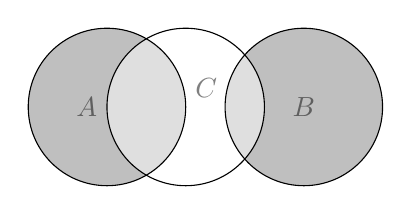
\begin{tikzpicture}
                \begin{scope}[shift={(3cm,-5cm)}, fill opacity=0.5]
                    \fill[gray] (0,0) circle (1);
                    \fill[gray] (2.5,0) circle (1);
                    \fill[white] (1,0) circle (1);
                    \draw (0,0) circle (1) node [left] {$A$};
                    \draw (2.5,0) circle (1) node {$B$};
                    \draw (1,0) circle (1) node [above right] {$C$};
                \end{scope}
            \end{tikzpicture}
    \end{enumerate}
    \textbf{2.10}
        \begin{enumerate}
            \item $S = \{NNN, NNF, NFN, NFF, FNN, FNF, FFN, FFF\}$
            \item $E = \{NFF, FNF, FFN, FFF\}$
            \item The second river is always safe to fish.
        \end{enumerate}
    \textbf{2.14}\\
    \textbf{2.16}\\
    \textbf{2.22}\\
    \textbf{2.26}\\
    \textbf{2.28}\\
    \textbf{2.30}\\
    \textbf{2.34}\\
    \textbf{2.38}\\
    \textbf{2.46}\\
    \textbf{2.50}\\
    \textbf{2.52}\\
    \textbf{2.56}\\
    \textbf{2.58}\\
    \textbf{2.64}\\
    \textbf{2.74}\\
    \textbf{2.80}\\
    \textbf{2.86}
    \begin{enumerate}
        \item fill
        \item fill
    \end{enumerate}
    \textbf{2.90}\\
    \textbf{2.92}\\
    \textbf{2.96}\\
    \textbf{2.98}\\
    \textbf{2.104}\\
    \textbf{2.118}\\
    \textbf{2.124}\\
    
\end{document}